\chapter{Construção}
\label{chap:Construcao}

Para a construção do \emph{software} aplicativo, foi utilizado uma arquitetura em
três camadas: sensor, distribuidor de acesso (\emph{IoT gateway}) e apresentação
(\emph{Web}). Nesta divisão, os sensores capturam as informações dos dispositivos
e repassam para a camada seguinte, no \emph{gateway} todas as partes se
encontram para fornecer e solicitar informações e, por último, a camada de
apresentação coleta o que é enviado dos sensores e gera uma página \emph{Web}
para visualização dos dados capturados.

Esta divisão está de acordo com o padrão encontrado em outras aplicações
\emph{IoT} onde a última camada usualmente varia entre apresentação e mineração
de dados (\emph{Data Mining}).

A camada de sensor utilizou as tecnologias \emph{Node.js}, \emph{TShark} parte
do \emph{Wireshark} e \emph{MQTT.js}. A camada \emph{gateway} foi composta
basicamente pelo \emph{MQTT Broker} \emph{Mosquitto}. Por fim a camada de
apresentação utlizou as tecnologias \emph{Node.js}, \emph{MQTT.js}, \emph{html},
\emph{css}, \emph{javascript}, \emph{Bootstrap} e \emph{Google Maps API}.

\begin{figure}[htb]
	\caption{\label{fig-arq-app}Arquitetura da aplicação}
	\begin{center}
		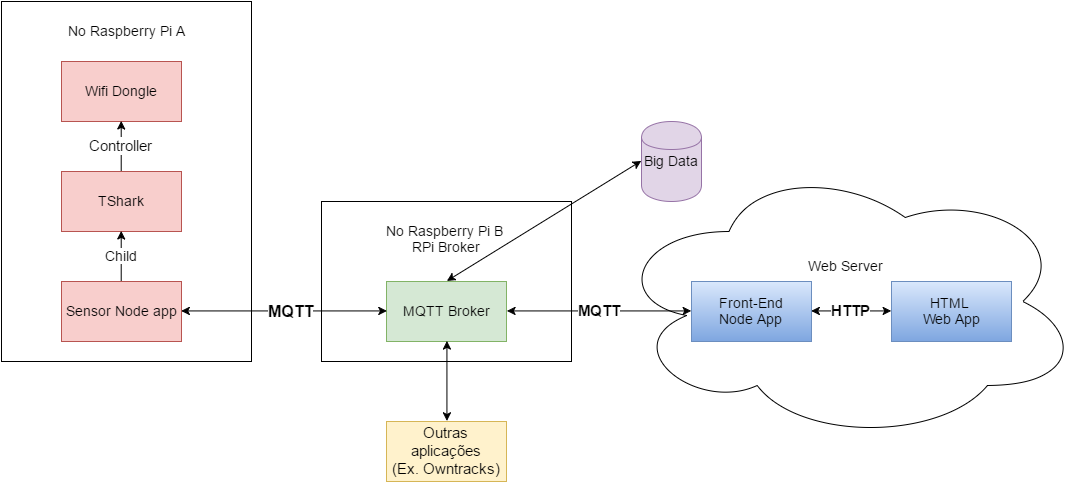
\includegraphics[width=1\textwidth]{050-construcao/esquema-proj.png}
	\end{center}
	\legend{Fonte: Elaborada pelo autor}
\end{figure}


\section{Sensor}
\label{sec:app-sensor}


A aplicação sensor tem como requisitos funcionais capturar, avaliar e classificar pacotes de
\emph{Wi-Fi}, inferir estatísticas de dispositivos e fornecer estas informações para
os interessados através do \emph{gateway}.

Para fazer a captura dos pacotes na aplicação final, diferente do que foi
demonstrado na \autoref{subsec:testes-rpi}, em especial o \emph{airodump-ng} e
sua interface demonstrada na \autoref{fig-airodump}, foi utilizado o programa
\emph{TShark} cujo modo de operação serve melhor para a construção dos
\emph{Streams} que serão abordados em breve.

\begin{citacao}

	TShark é uma versão orientada ao terminal do Wireshark projetada para capturar
	e exibir pacotes quando uma interface de usuário interativa não é necessária ou
	disponível. Ele suporta as mesmas opções como wireshark. \

	\citeonline{tshark} Tradução Nossa.
\end{citacao}

Como foi estabelecido no capítulo anterior, \emph{TShark}  utiliza a saída
padrão  do terminal (\emph{stdout}) como sua saída principal, esta
característica foi explorada com a aplicação \emph{nodejs}. Mais especificamente,
com o módulo \emph{child\_process},  que provê uma API que permite a criação e
controle de processos filhos do processo \emph{nodejs}.

\begin{citacao}

	Node.js é uma estrutura em tempo de execução construida sobre o motor de
	execução JavaScript V8 do Chrome. Node.js utiliza um modelo orientado a
	evento, de entrada e saída não bloqueante que o faz leve e eficiente.
	O ecosistema de pacotes do Node.js, npm, é o maior ecossistema de bibliotecas
	de código livre no mundo. \

	\citeonline{nodejs} Tradução Nossa.
\end{citacao}

Como também foi estabelecido anteriormente, o \emph{TShark} é executado com o
comando e argumentos como mostrado a seguir, a diferença em relação aos testes e
na escolha da plataforma é a forma de execução, na maneira mostrada, o processo é
criado utilizando o módulo \emph{child\_process} \cite{child_process} e os
argumentos são passados como um vetor (\emph{Array}).

\begin{lstlisting}[language=java]
const spawn = require('child_process').spawn;
const tsharkProcessoFilho = spawn(
	'tshark', [
		'-I',
		'-i', childIface,
		'-T', 'fields',
		'-E', 'separator=,',
		'-E', 'quote=d',
		'-e', 'wlan.sa',
		'-e', 'wlan.sa_resolved',
		'-e', 'wlan.ta',
		'-e', 'wlan.ta_resolved',
		'-e', 'radiotap.dbm_antsignal',
		'-e', 'wlan_mgt.ssid',
		'-Y', 'wlan.sa'
	]);
\end{lstlisting}

Para utilizar o resultado gerado pelo \emph{TShark}, utilizou-se outro método do
módulo \emph{child\_process} juntamente com a estrutura de \emph{Stream}
\cite{stream} que provê o método \emph{pipe(destination[, options])} que permite,
de maneira análoga ao operador '|' no terminal também chamado de \emph{pipe},
redirecionar a saída de um processo ou \emph{stream} de leitura para outro
processo ou \emph{stream} de escrita.

Com isso, ainda falta um \emph{stream} de escrita que receba a saída do
\emph{TShark} que foi definida no formato CSV. Para isso, uma biblioteca extra,
\emph{fast-csv}, deve ser instalada. Com ela, pode-se criar o \emph{stream}
necessário e configurá-lo para interpretar os resultados \cite{fast-csv}.

\begin{lstlisting}[language=java]
const csv = require("fast-csv");
let csvStream = csv()
  .on("data", function(data){
    let packet = new Packet(
      data[0], // sender address
      data[1], // sender address resolved
      data[2], // transmitter address
      data[3], // transmitter address resolved
      data[4], // potencia de sinal (rss)
      data[5], // nome da rede no pacote Beacon
    );
    processarPacote(packet);
  })
  .on("end", function(){
    console.log("done with tshark");
  });

tsharkProcessoFilho.stdout.setEncoding('utf8');
tsharkProcessoFilho.stdout.pipe(csvStream);
\end{lstlisting}

Nesta última linha, pode-se observar a operação de redirecionamento (\emph{pipe})
de \emph{stream} da saída padrão do processo filho (\emph{stdout}) para o
\emph{stream} de escrita descrito e configurado com o \emph{fast-csv}. A parte
faltante é o processamento dos pacotes e envio das inferências do sensor para o
\emph{gateway}.

Para as inferências e estatísticas, foi criado um objeto para armazenamento indexado
pelo endereço MAC e uma classe onde as informações
sobre cada dispositivo são agregadas. Desta forma, cada novo pacote pode ser acrescentado ao
histórico de cada dispositivo.

\begin{lstlisting}[language=java]
let devices = {};	// lista indexada de dispositivos

class Device {
  [...]
  appendPacket(packet){
    let curTime = ( new Date() ).toISOString();
    this.rssHistory.push(packet.radiotap.dbm_antsignal);
    this.ssidHistory[packet.wlan_mgt.ssid] = curTime;
    this.taHistory[packet.wlan.ta] = {
      ta      : packet.wlan.ta,
      ta_resolved  : packet.wlan.ta_resolved,
    };
  }
}

function processarPacote(packet) {
  let sa = packet.wlan.sa;
  if (! devices[sa]){
    devices[sa] = new Device(sa, packet.wlan.sa_resolved);
  }
  devices[sa].appendPacket(packet);
}
\end{lstlisting}

A partir desta lista, é posível calcular a média e o desvio padrão de potência de
sinal para cada dispositivo descoberto.


\begin{lstlisting}[language=java]
class Device {
  [...]
  get rssStatistics(){
    let sum = 0;
    let avg = 0;
    let variance = 0;
    let stdDeviation = 0;
    if (this.rssHistory.length > 0){
      for (let rss of this.rssHistory){
        sum += rss;
      }
      avg = sum / this.rssHistory.length;

      sum = 0;
      for (let rss of this.rssHistory){
        sum += Math.pow(( rss - avg ), 2);
      }
      variance = sum / (this.rssHistory.length - 1);
      stdDeviation = Math.sqrt(variance);
    }
    return {
      size      : this.rssHistory.length,
      avg        : avg,
      variance    : variance,
      stdDeviation  : stdDeviation,
      time      : ( new Date() ).toISOString(),
    };
  }
}
\end{lstlisting}

Por fim, é necessário comunicar aos interessados nessas inferências, o que é
feito através do módulo \citeonline{mqttjs}.

\begin{lstlisting}[language=java]
const mqtt = require('mqtt');
const mqttBrok = `mqtt://${config.mqttHost}:${config.mqttPort}`;
let clientMqtt  = mqtt.connect(mqttBrok, {
  username  : config.mqttUser,
  password  : config.mqttPwd,
})
clientMqtt.on('connect', function () {
  clientMqtt.subscribe('devices');
  startTshark();
});
clientMqtt.on('message', function (topic, message) {
  if (topic.toString() == 'devices') {
    switch (message.toString()) {
    case 'list':
      clientMqtt.publish(
        'devices/report',
        JSON.stringify( tshark.getDevices() )
      );
      break;
    case 'report':
      clientMqtt.publish(
        'devices/report',
        JSON.stringify( tshark.getReport() )
      );
      break;
    default:
      let mac = message.toString();
      clientMqtt.publish(
        'devices/report',
        JSON.stringify( tshark.getDeviceReport(mac) )
      );
      break;
    }
  }
});
\end{lstlisting}

No caso desta listagem de código, quando a aplicação é iniciada ela conecta-se ao \emph{MQTT Broker}.
Quando a conexão é estabelecida, ela solicita ao \emph{MQTT Broker} a inscrição
para receber as publicações no tópico 'devices' e o processo filho \emph{TShark}
é iniciado. O processo filho é executado, os resultados são capturados e
guardados.

Quando uma mensagem no tópico 'devices' é recebida, três reações podem acontecer:
a lista de dispositivos deve ser fornecida, o relatório do sensor deve ser
fornecido ou um relatório sobre um dispositivo específico deve ser fornecido.
Para todos os casos, uma resposta adequada é imediatamente processada e enviada
para o tópico 'devices/report'.

Em conclusão, a aplicação sensor instancia o processo de aquisição de dados
\emph{TShark} assincronamente e captura, classifica e armazena todos os pacotes
que ficam acessíveis através de requisições ao tópico \emph{MQTT} 'devices'.
Isso cobre os requisitos funcionais desta aplicação.

//IMAGEM MQTT DASHBOARD --> coloca um paragrafo antes para explicar

Os requisitos não-funcionais desta aplicação estão ligados com o ambiente de
implantação que é um RPI3 remoto, sem outro dispositivo de entrada e saída
exceto a comunicação \emph{MQTT}, portanto, sem nenhum aspecto permitindo
monitoração de um humano que garanta que o aplicativo continue funcionando.

Este ambiente se assemelha muito a aplicações em núvem, onde não há acesso
físico ao computador onde a aplicação é executada. Neste ambiente, procura-se
garantir que a aplicação seja executada constantemente e atualizada
automaticamente sempre que uma nova versão é construída e testada. Estas
garantias podem ser alcançadas com ferramentas de integração contínua
(\emph{Continuous Integration} - CI). No caso do Github, a escolha de hospedagem
de código deste projeto, diversas opções deste tipo de ferramenta podem ser
encontradas em \cite{githubdeploy}.

No entanto, para esta aplicação, construiu-se uma solução extremamente
simplificada destas ferramentas utilizando a arquitetura existente do programa
\emph{git} para garantir que novas versões fossem instaladas assim que possível.
A implementação consiste da adição, nas primeiras instruções do aplicativo,
uma rotina que executa sincronamente um programa externo através do terminal
(diferente da execução do \emph{TShark} que é assíncrona). Este programa é
o \emph{git} com a opção \emph{pull} que, quando executado em um diretório que
é repositório, solicita ao servidor configurado, como \emph{origin}, a atualização
do código do \emph{branch} atual. Se a mensagem encontrada na saída padrão
(\emph{stdout}) resultante deste comando for diferente de
\emph{"Already up-to-date."}, o programa finaliza imediatamente, pois uma nova
versão foi baixada e uma reinicialização da aplicação é necessária.
Em resumo, uma vez instalada a aplicação utilizando a ferramenta \emph{git}, ela
será atualizada com o mesmo processo com que foi instalada.

O outro requisito é que a aplicação seja executada constantemente. Para isso,
pode-se utilizar uma aplicação também escrita em \emph{Node.js} e disponível no
gerenciador de pacotes \emph{npm}: \emph{forever-service}. Ela registra um novo serviço no sistema operacional
linux para que a infra-estrutura de gerenciamento de serviços  existente seja
aproveitada (por exemplo: início automático após o início do sistema). Além disso, a sua dependência
\emph{forever} garante que a aplicação seja reinicializada sempre que finaliza,
executando a aplicação constantemente \cite{forever-service}.


\section{Gateway}
\label{sec:app-gw}

\begin{citacao}

	Eclipse Mosquitto™ é um distribuidor de mensagens de código aberto (EPL/EDL
	licenciado) que implementa o protocolo MQTT versões 3.1 e 3.1.1. O MQTT
	fornece um método leve de transmitir mensagens usando um modelo de
	publicação/inscrição. Isso o torna adequado para mensagens "Internet das
	Coisas", como com sensores de baixa potência ou dispositivos móveis, como
	telefones, computadores embutidos ou microcontroladores como o Arduino. \

	\citeonline{mosquitto} Tradução Nossa.
\end{citacao}


\section{Apresentação Web}
\label{sec:app-web}


\begin{figure}[htb]
	\caption{\label{fig-web-app}Web APP}
	\begin{center}
		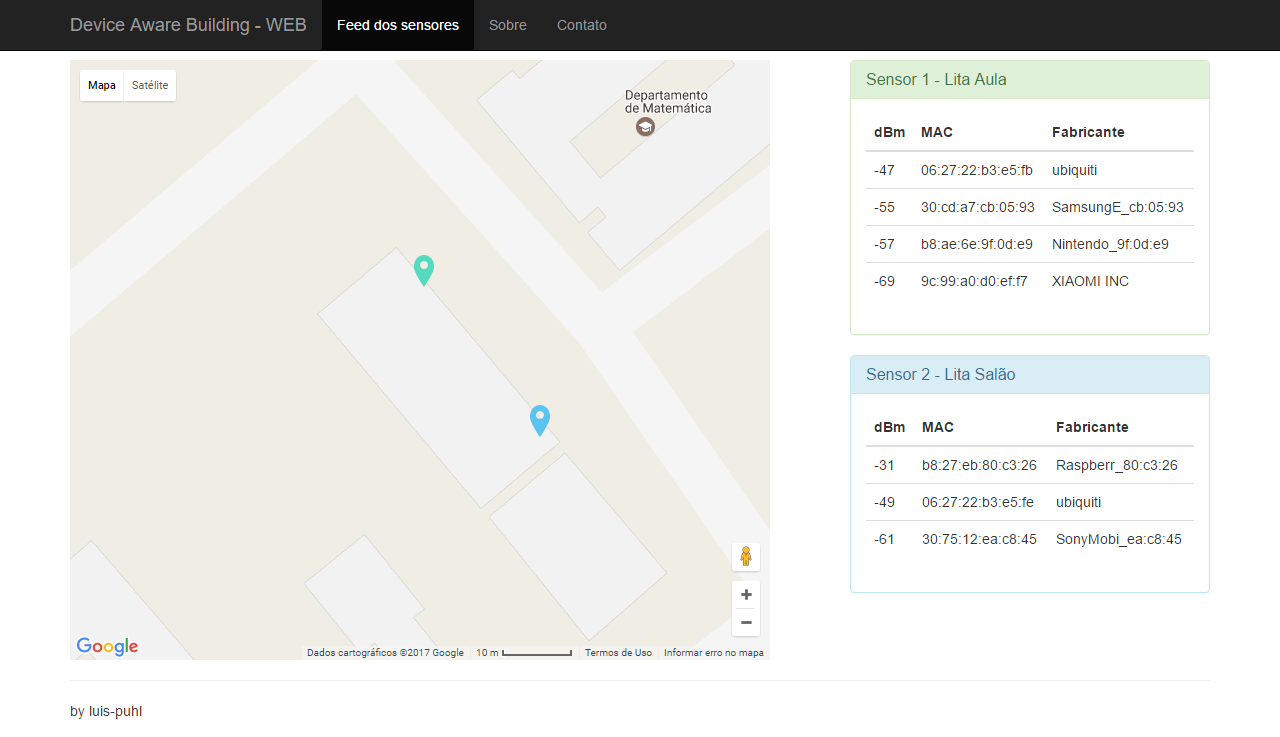
\includegraphics[width=1\textwidth]{050-construcao/web-app.png}
	\end{center}
	\legend{Fonte: Elaborada pelo autor}
\end{figure}
